\documentclass[12pt]{article}
\parindent0em
\parskip 1ex plus 0.4ex minus 0.4ex

%%%%%%%%%%%%%%%%%%%%%%%%%%%%%%%%%%%%%%%%%%%%%%%%%%%%%%
%                   Packages                         %
%%%%%%%%%%%%%%%%%%%%%%%%%%%%%%%%%%%%%%%%%%%%%%%%%%%%%%
\usepackage[a4paper,vmargin=30mm,hmargin=25mm]{geometry}
\usepackage{polyglossia}
\setdefaultlanguage{german}
\usepackage{fontspec}
\usepackage{hyperref}
\usepackage[font=small,labelfont=bf]{caption}
\usepackage{lipsum}
\usepackage[table]{xcolor}
\usepackage{sectsty}
\usepackage{array}
\usepackage{tabularx,stackengine,collcell}
\usepackage{listings}
\usepackage{todonotes}
\usepackage{graphicx}

%%%%%%%%%%%%%%%%%%%%%%%%%%%%%%%%%%%%%%%%%%%%%%%%%%%%%%
%                   Link-Setup                       %
%%%%%%%%%%%%%%%%%%%%%%%%%%%%%%%%%%%%%%%%%%%%%%%%%%%%%%
\hypersetup{
    colorlinks = true,
    linkbordercolor = {white},
    linkcolor = {blue}
}
\usepackage{graphicx}

%%%%%%%%%%%%%%%%%%%%%%%%%%%%%%%%%%%%%%%%%%%%%%%%%%%%%%
%             Insert Graphic Command                 %
%%%%%%%%%%%%%%%%%%%%%%%%%%%%%%%%%%%%%%%%%%%%%%%%%%%%%%
\graphicspath{ {./images/} }
\newcommand{\graphic}[2]{
\captionsetup{type=figure}
\begin{center}
\includegraphics[width=0.95\textwidth,height=0.75\textheight,keepaspectratio]{#1}
\end{center}
\captionof{figure}{#2}
\bigskip
}

%%%%%%%%%%%%%%%%%%%%%%%%%%%%%%%%%%%%%%%%%%%%%%%%%%%%%%
%             	   Fonts & Colors                    %
%%%%%%%%%%%%%%%%%%%%%%%%%%%%%%%%%%%%%%%%%%%%%%%%%%%%%%
\renewcommand{\familydefault}{\sfdefault}
\definecolor{DarkBlue}{rgb}{0.212,0.373,0.576}
\definecolor{LightBlue}{rgb}{0.318,0.506,0.741}
\definecolor{TableBlue1}{rgb}{0.855,0.933,0.953}
\definecolor{TableBlue2}{rgb}{0.929,0.965,0.976}
\definecolor{grey}{rgb}{0.302,0.333,0.361}

\sectionfont{\rmfamily\color{DarkBlue}}
\subsectionfont{\rmfamily\color{LightBlue}}
\subsubsectionfont{\rmfamily\color{LightBlue}}

\newcommand{\method}[1]{
{\color{grey}#1}
}

%%%%%%%%%%%%%%%%%%%%%%%%%%%%%%%%%%%%%%%%%%%%%%%%%%%%%%
%               Insert Table Command                 %
%%%%%%%%%%%%%%%%%%%%%%%%%%%%%%%%%%%%%%%%%%%%%%%%%%%%%%

\renewcommand*{\arraystretch}{1.5}
\newcolumntype{L}[1]{>{\bf\raggedright\let\newline\\\arraybackslash}m{#1}}
\newcolumntype{C}[1]{>{\raggedright\let\newline\\\arraybackslash}m{#1}}

\newbool{firstline}
\newenvironment{atab}
{\leavevmode\newline\newline
\rowcolors{2}{TableBlue1}{TableBlue2}
\begin{tabular*}{0.75\textwidth}[t]{L{3cm}C{13cm}}
 & \\
}{\end{tabular*}}

\newenvironment{btab}
{\newcommand{\h}[1]{$\makebox[\linewidth]{\textbf{##1}}$}\leavevmode\newline\newline
\rowcolors{2}{TableBlue1}{TableBlue2}
\begin{tabular*}{0.75\textwidth}[t]{C{16cm}}
\\
}{\end{tabular*}}
%%%%%%%%%%%%%%%%%%%%%%%%%%%%%%%%%%%%%%%%%%%%%%%%%%%%%%
%             	     Title page                      %
%%%%%%%%%%%%%%%%%%%%%%%%%%%%%%%%%%%%%%%%%%%%%%%%%%%%%%

\begin{document}

\title{\begin{center}\fontsize{40bp}{40bp}\selectfont\color{DarkBlue}
Cloud and Distributed Computing Dokumentation \\ [20pt]
\color{black}
\fontsize{16bp}{16bp}\selectfont
\fontsize{30bp}{30bp}\selectfont
\color{LightBlue}
LoL Stats Website\\
\fontsize{10bp}{10bp}\selectfont
\color{black}
\bigskip
\end{center}
}
\maketitle

\date{}
\begin{center}
\textbf{\fontsize{12bp}{12bp}\selectfont
Autoren:\\}
\bigskip
\author{xxxxx Julian Sobott\\ 
\and	 76514 Christian Greiner\\
\and 75977 Shadrach Arulrajah Patrick\\
\and 75981 Tim Staudenmaier
}
\end{center}
\begin{figure}
\centering

\includegraphics[width=0.75\textwidth]{HSAalenLogo}
\end{figure}

\newpage
			
%%%%%%%%%%%%%%%%%%%%%%%%%%%%%%%%%%%%%%%%%%%%%%%%%%%%%%
%             	  Tabel of contents                  %
%%%%%%%%%%%%%%%%%%%%%%%%%%%%%%%%%%%%%%%%%%%%%%%%%%%%%%  

\setcounter{page}{1} % Seitenzahl der zweiten Seite auf 1 setzen

{\hypersetup{linkcolor=black}
\tableofcontents
}
\newpage

%compile with XeLaTeX

%\begin{atab}
% row1.1 & row1.2 \\
% row2.1 & row2.2 \\
% ...
%\end{atab}

%\graphic{filename}{caption}

%colors: DarkBlue, LightBlue, TableBlue1, TableBlue2

%hyperlinks:
%Link target: \hypertarget{targetname}{}
%Clickable Link: \hyperlink{targetname}{text}

%\section{name} for 3 main sections
%\subsection{name} and \subsubsection{name}

%%%%%%%%%%%%%%%%%%%%%%%%%%%%%%%%%%%%%%%%%%%%%%%%%%%%%%
%%%%%%%%%%%%%%%%%%%%%%%%%%%%%%%%%%%%%%%%%%%%%%%%%%%%%%
%             	  Begin of Document                  %
%%%%%%%%%%%%%%%%%%%%%%%%%%%%%%%%%%%%%%%%%%%%%%%%%%%%%%
%%%%%%%%%%%%%%%%%%%%%%%%%%%%%%%%%%%%%%%%%%%%%%%%%%%%%%

% template: https://docs.arc42.org/home/

\section{Einführungen und Ziele}
\subsection{Ziel}

Lol-Stats ist eine Webanwendung, die speziell für aktive "League of Legends"-Spieler entwickelt wurde. Ihre Hauptfunktionalität liegt in der Berechnung und Vermittlung
von Statistiken, die innerhalb der Spielrunden erfasst werden. Bei den Statistiken handelt sich nicht nur um übliche, simple Daten, sondern vielmehr um spezielle Errungenschaften, die es so nicht auf anderen Webseiten gibt. 
Lol-Stats bietet außerdem die Möglichkeit, diese Errungenschaften mit denen anderer Spieler zu vergleichen. Man kann bestimmte Spieler auch als Konkurrenten hinzufügen, um sich schneller und einfacher mit ihnen zu vergleichen.\\
Zudem kann man sich mit der gesamten Gruppe an ausgewählten Konkurrenten oder der globalen Liste an Spieler vergleichen.

\subsection{Anforderungen}

\subsubsection{Technisch}

Die gesamte Architektur soll dabei geschickt in Services aufgeteilt werden, wobei jeder Service in seinem eigenen Docker-Container laufen soll.
Ebenso gibt es kein zentrales Datenbanksystem, denn jeder Service soll, wenn sinnvoll, über eine eigene Datenbank verfügen.\\
Das Backend ist dafür zuständig die Daten aus der Riot API zu importieren und dem Frontend zur Verfügung zu stellen. Dazu muss eine Schnittstelle zwischen der Riot API und dem Backend, sowie zwischen Backend und Frontend geschaffen werden. Des weiteren existiert ein Servive zur Verwaltung der User-Accounts, welcher ebenfalls mit dem Frontend kommunizieren muss.\\
In dieser Anwendung soll es unter anderem Echtzeitverarbeitung von Daten geben. 
Das Frontend soll eine Benutzerschnittstelle implementieren, die Responsiveness und Intuitivität aufweist, sodass der Umgang mit der Website für Benutzer möglichst einfach ist.

\subsubsection{Fachlich}

\begin{itemize}
    \item Als Nutzer will ich die Achievements von meinem gewünschten Account sehen können.
    \item Als Nutzer will ich meine Achievements mit den Achievements beliebiger Spieler, global oder mit Ranks vergleichen können.
    \item Als Nutzer will ich beliebige Spieler zu meinen Favoriten hinzufügen oder löschen können.
    \item Als Nutzer will ich mich speziell nur mit diesen Favoriten vergleichen können.
    \item Als Nutzer will ich meine zuletzt gespielten Spiele ansehen können.
    \item Als Nutzer will ich globale, zufällige Statistiken sehen können, auch wenn ich nicht angmeldet bin.
\end{itemize}


\section{Randbedingungen}

\subsection{Riot API Ratelimits}\label{riot-api-ratelimits}
Für die API von Riot Games gibt es zwei verschiendene API Keys. Den Development Key und den Production Key. Einen Development Key kann hier jeder beantragen, für einen Production Key hingegen muss ein bereits fertiges Produkt vorhanden sein, welches dann noch durch einen Application Prozess angenommen werden muss.\\
Mit einem Production Key sind 500 Request alle 10 Sekunden bzw. 30.000 Requests alle 10 Minuten erlaubt.\\
Für dieses Projekt wird ein Development Key verwendet. Für diesen sind die Ratelimits deutlich geringer, mit 20 Requests pro Sekunde bzw. 100 Requests alle 2 Minuten.\\
Für die Demonstration dieses Projekts sind aber auch diese deutlich geringeren Ratelimits ausreichend, da nie mehr als 1-2 Leute gleichzeitig auf die Website zugreifen und die Anzahl der gespeicherten Spieler gering bleibt.\\
Möchte man die Website später öffentlich zugänglich machen, so müsste ein Production Key verwendet werden, da Riot es nicht erlaubt Development Keys für öffentliche Produkte zu verwenden und die Ratelimits nicht ausreichend währen.

\subsection{Server Performance}

Als Infrastruktur wurde der Landesdienst von bwCloud verwendet, der eine kostenlose
"Infrastructure-as-a-Service" Umgebung für Forschung und Lehre in Baden-Württemberg bereitstellt.
Wie Grafik nachfolgende Grafik zeigt, kann pro Nutzer nur ein bestimmtes Kontingent an VCPUS, RAM sowie Datenträger-Speicher verwendet werden.
Sobald mehr Server-Ressourcen benötigt werden, ist dies nicht möglich ohne auf einen kostenpflichtigen Dienst wechseln zu müssen.

\graphic{uebersicht_kontingente.png}{Übersicht der verfügbaren Kontigente}

Diese beschränkten Ressourcen haben einen direkten Einfluss auf die Ausführung von komplexen Datenbankoperationen. Außerdem ist ein
horizontales Scaling des Dienstes durch die Limitierung ebenso nicht möglich, wodurch die Performance nur durch verbesserte SQL-Abfragen
optimiert werden kann.

\section{Context and Scope}
external communication partners (specify external interfaces)
Show and explain context diagram with clear system boundaries and external systems \& actors (e.g., users). Other services should be seen in this context. Looks like a Use Case Diagram without the Use Cases in the System, the actors show their forms of communication with.

\subsection{Context Diagram}

\subsection{Riot API}
\subsubsection{Cassiopeia}

\subsubsection{Riot Watcher}
\section{Lösungsstrategie}

\subsection{Service-Diagramm}

\begin{figure}
    \centering
    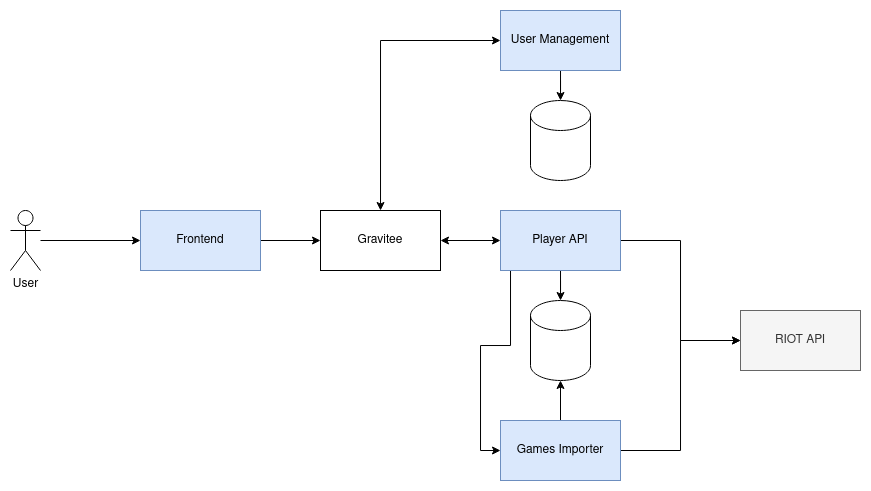
\includegraphics[width=\textwidth]{images/cdc-05-service-diagram.drawio}
    \caption{Service Diagramm der Applikation}
    \label{fig:service-diagram}
\end{figure}

In Abbildung~\ref{fig:service-diagram} ist das Service Diagramm für die Applikation zu sehen.
Es gibt ein Frontend, dass über ein zentrales API Gateway mit den Backend Services kommuniziert.
Als API Gateway wird Gravitee verwendet.
Der User Management Service ist für das verwalten von Usern auf der Webseite verantwortlich.
Hierfür hat der Service seine eigene PostgreSQl Datenbank.
Die Player API stellt eine Schnittstelle zur LoL Datenbank zur Verfügung.
Hierüber werden alle Daten zur Verfügung gestellt, die Spielinformationen benötigen.
Außerdem kommuniziert die Player API direkt mit dem Games Importer Service um das Importieren von Spielern zu triggern.
Der Games Importer Service schreibt alle Daten in die geteilte LoL Datenbank, welches ebenfalls eine PostgreSQl Datenbank ist.
Um an die Daten zu kommen, fragt der Games Importer Service die externe Riot API an.

\subsection{Technolgien}

\subsubsection{Games Importer}\label{subsubsec:games-importer}
Dieser Service ist die Verbindung zwischen der Riot API und unserer Anwendung. Er läuft in seinem eigenen Docker Container. Hier werden die Daten aus der Riot API abgefragt und dann in unserer Datenbank gespeichert.\\
Der Service ist in Python geschrieben, da hierfür bereits Libraries zur Kommunikation mit der Riot API vorhanden sind (siehe \ref{riot-api-libraries}).\\
Neben den Riot API Wrappern Cassiopeia und Riot Watcher wird noch das psycopg2 Package verwendet, welches Zugriff auf die PostgreSQL Datenbank bietet. Psycopg2 erlaubt es in Python SQL Statements zu bauen und auszuführen um somit die Daten von der Riot API in der Datenbank zu speichern.\\
Der Games Importer Service läuft dauerhaft und aktualisiert in 5min Abständen alle in der Datenbank gespeicherten Spieler. \\
Des weitere läuft in deinem weiteren Thread eine GRPC Connection, welche es erlaubt den Import eines neuen Spieler anzufragen. Dieser wird dann erstmals von der Riot API in die Datenbank importiert und bei den zukünftigen Updates berücksichtigt.

\subsubsection{LoL Database}
Die PostgreSQL Datenbank läuft in einem eigenen Docker Container. In dieser Datenbank werden alle Spieler bezogenen Daten gespeichert, welche auf der Website angezeigt werden.\\
Die Daten werden alle vom Games Importer Service aus der Riot API gelesen und in dieser Datenbank gespeichert. Der Player API Service kann dann auf diese Daten zugreifen um sie an das Frontend weiterzugeben.

\subsubsection{Player API}

Dieser Service stellt die importierten Daten des Service~\ref{subsubsec:games-importer} dar.
Als Programmiersprache um eine schnelle Entwicklung zu erreichen und um im Backend nur eine Sprache zu verwenden.
Als Webframework wurde sich für FastAPI entschieden, aufgrund der hohen Performance.
Für den Datenbankzugriff wurde sich für SQLAlchemy entschieden, um ein ORM verwenden zu können.

\subsubsection{User Management}

Im Bereich des User Managements werden Daten vom Nutzer gespeichert, die für die eigene Plattform relevant sind. Dieser Service bietet u.a. Funktionen um Accounts zu erstellen oder zu löschen.\\
Dieser Backend-Service wurde in Python mit Flask geschrieben.
Für das Mapping der Daten wurde SQLAlchemy genommen und die Speicherung findet in einer PostgreSQL-Datenbank statt.    

\subsubsection{Frontend}

Über das Frontend lässt sich die Anwendung benutzen. Sie ist derzeit für die Benutzung mit dem Webbrowser ausgelegt. Dabei kommen folgende Technolgien zum Einsatz.  \\

\textbf{NuxtJS} \\

Für die Umsetzung des reaktiven Frontends wurde das "NuxtJs"-Framework (\href{https://nuxtjs.org/}{https://nuxtjs.org/}) entschieden. Dieses erlaubt es komplexe Vue-Anwendungen umzusetzen und unterstützt Entwickler:innen
bei unterschiedlichen Problemstellungen der Frontend-Entwicklung. Aufgrund bereits existierender Erfahrung mit Vue und dem Framework viel die Wahl auf diese Technologie.
Dadurch ist eine rasche Entwicklung gewährleistet, indem die Einarbeitungszeit in neue Technologien wegfällt. Die Kommunikation mit verschiedenen Diensten passiert
über das HTTP-Protokoll. Mit dem eingebauten Modul "Axios", welches als HTTP-Client dient, werden HTTP-Anfragen an das Backend gesendet, um die entsprechenden Daten 
zu erhalten. Zur Authentifizierung der Benutzer:innen wird das Modul "NuxtJs Auth" (\href{https://auth.nuxtjs.org/}{https://auth.nuxtjs.org/}) verwendet. Dieses stellt eine API zur Verfügung, mit der Registierungs- und Anmeldeprozess durchgeführt werden kann.
Ebenso übernimmt es die Speicherung und Verifizierung des vom User-Backend erhaltene JWT-Token. \\

\textbf{Design} \\

Um ein einfache, responsive und übersichtliche Web-Oberfläche den Nutzer:innen zu gewährleisten, viel die Wahl auf "Tabler" (\href{http://tabler.io/}{http://tabler.io/}). Dies ist ein freies Frontend-CSS-Framework
und stellt das Grundgerüst einer Administrationsoberfläche zur Verfügung. Aufgrund zahlreicher HTML-Module kann die Benutzeroberfläche nach Belieben konzeptioniert und 
umgesetzt werden. Ebenso bietet diese CCS-Framework bereits ein responsives Layout, wodruch zeitgleich die Benutzeroberfläche automatisch für mobile Endgeräte angepasst wird.

\subsection{Architektur}

In den beiden Tabellen~\ref{tab:goals} und~\ref{tab:principles}, werden die Ziele der Architektur aufgelistet
und die jeweiligen Architektur Prinzipien, die diese unterstützen.

\subsubsection{Architektur Ziele}
\begin{center}
    \begin{tabular}{|l|l|l| p{5cm} |p{2.5cm}|}
        \hline
        \textbf{Priorität} & \textbf{Arch. Ziel (AG)} & \textbf{Abkürzung} & \textbf{Eigenschaften} & \textbf{Unterstützt von APs?} \\
        \hline
        1 & Funktionalität & AG:FUNC & UI, Business Logik, Daten & AP:SOA \\
        2 & Benutzbarkeit & AG:USA & responsive ui &  \\
        3 & Portabilität & AG:PORT & DB, OS Unabhängigkeit & AP:PY AP:DOCKER AP:ORM\\
        4 & Interoperabilität & AG:INT & RDB Austauschbarkeit & AP:ORM \\
        5 & Wartbarkeit & AG:MTN & & AP:SOA AP:PY AP:DOCKER AP:ORM\\
        6 & Performance & AG:PERF & Latenz & AP:POLL \\
        7 & Ausfallsicherheit & AG:RLB & ACID Transaktionen, unabhängige Services & AP:SOA AP:RDB AP:DOCKER\\
        8 & Security & AG:SEC & Passwörter hashen, Kommunikation über https &  \\
        \hline
    \end{tabular}
    \label{tab:goals}
\end{center}
\subsubsection{Prinzipien}

\begin{center}
    \begin{tabular}{|l|l| p{5cm} |p{3cm}|}
        \hline
        \textbf{Arch. Prinzip (AP)} & \textbf{Abkürzung} & \textbf{Beschreibung.} & \textbf{Unterstützt AGs} \\
        \hline
        Service orientiert & AP:SOA & Backends aufgeteilt auf Services um Requests zu händeln & AG:FUNC AG:MTN AG:RLB \\
        Relationale DB & AP:RDB & Daten in relationaler Datenbank mit SQL gespeichert & AG:RLB \\
        Python & AP:PY & Python ist OS unabhängig und ermöglicht gute Wartbarkeit & AG:PORT AG:MTN \\
        Docker & AP:DOCKER & Docker erlaubt unabhängiges und einfaches deployment & AG:MTN AG:PORT AG:RLB \\
        OR Mapping & AP:ORM & Datenbankunabhängigkeit und einfaches Entwickeln & AG:PORT AG:INT AG:MTN \\
        Polling & AP:POLL & Polling statt lang wartende Requests ermöglicht schnelle Antworten & AG:PERF \\
        \hline
    \end{tabular}
    \label{tab:principles}
\end{center}

\section{Bausteinsicht}

\subsection{Games Importer Service}
\subsubsection{Klassendiagramm}
\graphic{GamesImporter}{Klassendiagramm des Game Importer Service}
\subsubsection{Verantwortlichkeiten}
Dieser Service ist dafür zuständig, die benötigten Daten bei der Riot API anzufragen und dann in der LoL Datenbank zu speichern. Die Struktur des Services ist im obigen Klassendiagramm zu sehen. \\
Die db Klasse bietet alle Funktionen, um mit der Datenbank zu interagieren: neue Daten speichern, Daten lesen und Daten updaten. Dazu wird das psycopg2 Package verwendet.\\
Die App Klasse beinhaltet den main loop (update\_loop Funktion). In dieser werden dann weitere Funktionen aufgerufen, um alle Spieler zu updaten. Dazu werden zuerst die Methoden des summoner.py Moduls verwendet, welche einen einzelnen Spieler updaten können. In dieser Methode werden zunächst alle Daten des Summoners (Level, Name, ...) aktualisiert. Dann wird das matchhistory.py Modul verwendet, welches für den Spieler die MatchHistory importieren kann (add\_missing\_games\_tp\_db(db, get\_match\_ids(), puuid). Dieses verwendet dabei noch die Challenges Klasse, welche die Challenges für einzelne Spieler speichern kann (store\_challenges()). Dabei werden mithilfe der in der Datenbank vorhandenen Werte für total, average und highscore die neuen Werte berechnet und diese dann gespeichert.\\

Der PlayerImportRequest erbt von der von GRPC generierten Klasse ImporterService und ist für die Verbindung mit der PlayerAPI zuständig. Über diese Klasse kann eine Anfrage gesendet werden, um den Import eines neuen Spielers zu starten, wobei dann dieselbe Abfolge durchlaufen wird wie oben bereits beim updaten eines Spielers beschrieben.

\subsubsection{Externe Software}
\begin{itemize}

\item \textbf{GRPC:} \href{https://grpc.io/docs/languages/python/basics/}{https://grpc.io} Kommunikation zwischen Backend Services\\
\item \textbf{Cassiopeia:} \href{https://github.com/meraki-analytics/cassiopeia}{https://github.com/meraki-analytics/cassiopeia} Riot API Wrapper für Python\\
\item \textbf{Riot Watcher:} \href{https://github.com/pseudonym117/Riot-Watcher}{https://github.com/pseudonym117/Riot-Watcher} Riot API Wrapper für Python\\
\item \textbf{psycopg2:} \href{https://pypi.org/project/psycopg2/}{https://pypi.org/project/psycopg2/} Python library für Zugriff auf PostgreSQL Datenbanken \\
\item \textbf{Riot API:} \href{https://developer.riotgames.com/}{https://developer.riotgames.com/} API von Riot die Zugriff zu Daten über u.a. League of Legends bietet\\

\end{itemize}

\subsection{Player API}

\subsubsection{Komponentendiagramm}\label{subsubsec:player-api-component-diagram}

\begin{figure}
    \centering
    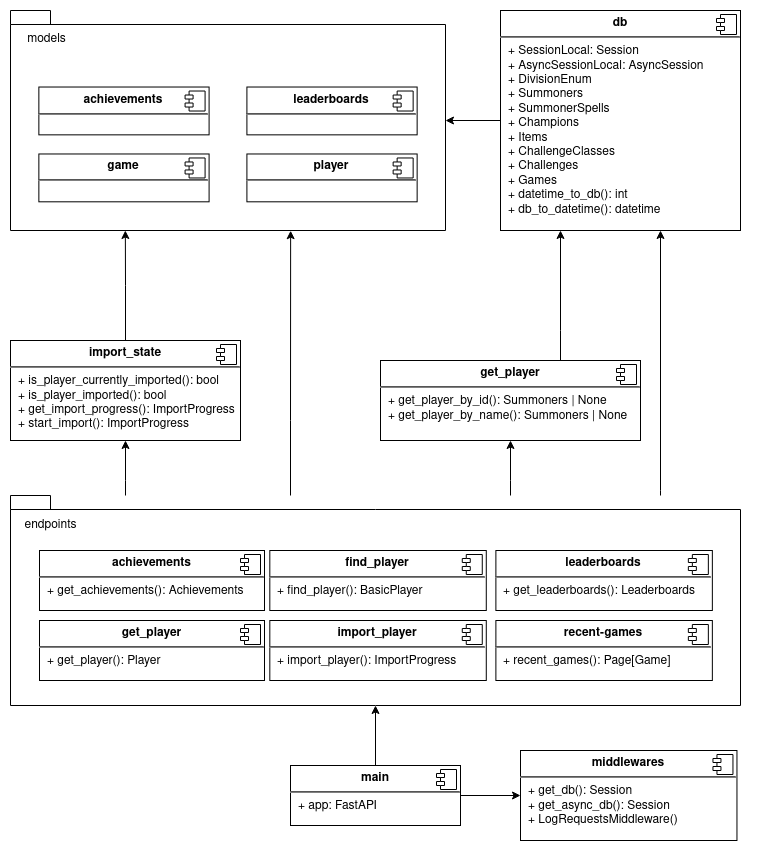
\includegraphics[width=\textwidth]{cdc-06-player-api-static.drawio}
    \caption{Komponenten Diagramm des PlayerAPI Services}
    \label{fig:player-api-component-diagram}
\end{figure}
Das in Abbildung~\ref{fig:player-api-component-diagram} abgebildete Komponenten Diagramm stellt die wichtigsten
Komponenten des PlayerAPI Services dar.
Wobei im \lstinline!model! Package nur die Module ohne die Klassen dargestellt werden, um das Diagramm
übersichtlich zu halten und es sich hierbei nur um Datenklassen handelt ohne Logik.

\subsubsection{Verantwortlichkeiten}

Dieser Service stellt folgende Endpunkte zur Verfügung:
\begin{itemize}
    \item \textbf{achievements}: Ein Spieler kann seine/ihre Challenges mit anderen Spielern vergleichen.
    \item \textbf{find\_player}: Prüft ob ein Spieler existiert.
    \item \textbf{leaderboards}: Stellt globale Highscore Listen zur Verfügung.
    \item \textbf{get\_player}: Stellt Informationen wie rank eines Spielers zur Verfügung
    \item \textbf{import\_player}: Triggert den Importprozess, falls Import noch nicht läuft.
    Gibt immer den aktuellen progress zurück.
    \item \textbf{recent\_games}: Stellt die zuletzt gespielten Spiele paginiert zur Verfügung.
\end{itemize}

Das \lstinline!main! Modul ist der Einstiegspunkt für die Applikation.
Hier wird die App mit den Routen konfiguriert, middlewares hinzugefügt und logging mit monitoring konfiguriert.

\lstinline!import_state! und \lstinline!get_player! haben Funktionen, die in fast jedem Endpunkt genutzt werden.

Im \lstinline!db! Modul ist das ORM Modell und die Verbindung zur Datenbank.

Das \lstinline!models! Package enthält Datenklassen, die keine Logik enthalten.
FastAPI wandelt diese in den Endpunkten automatisch in JSON um, wodurch alles typisiert ist.
Um das Diagramm übersichtlich zu halten, wurden nur die Module ohne die enthaltenen Klassen dargestellt.

\subsubsection{Externe Software}

\begin{itemize}
    \item \textbf{FastAPI} (\href{https://fastapi.tiangolo.com/}{https://fastapi.tiangolo.com/}): Web framework
    \item \textbf{pydantic} (\href{https://pydantic-docs.helpmanual.io/}{https://pydantic-docs.helpmanual.io/}): Datenklassen und Validierung
    \item \textbf{sqlalchemy} (\href{https://www.sqlalchemy.org/}{https://www.sqlalchemy.org/}): Datenbank ORM
    \item \textbf{GRPC} (\href{https://grpc.io/docs/languages/python/basics/}{https://grpc.io/docs/languages/python/basics/}): Kommunikation über GRPC
    \item \textbf{sentry} (\href{https://sentry.io}{https://sentry.io}): Fehler Überwachung fürs Monitoring
    \item \textbf{opentelemetry} (\href{https://opentelemetry.io/}{https://opentelemetry.io/}): Tracing fürs Monitoring
\end{itemize}

\subsection{User Management}
\subsubsection{Klassendiagramm}
\todo{User Management Klassendiagramm}
\subsubsection{Verantwortlichkeiten}
Zu den eigenen Daten des User Backends gehören unter anderem die Region oder die Referenz zu einem Lol-Account dazu, 
aber auch alle notwendige Daten, die bei der Registrierung und beim Login entstehen. Für die Validierung dieser einkommenden Daten wurde die Libaries "Werkzeug" und "Marshmallow" verwendet.
Außerdem beinhaltet dieser Service die Zuständigkeit für das Token und Competitor Management. So wurde für das Kreieren und Validieren der Tokens die Libary
"PyJWT" verwendet.
\subsubsection{Externe Software}
\begin{itemize}
\item \textbf{Flask} (\href{https://flask.palletsprojects.com/en/2.1.x/}{https://flask.palletsprojects.com/en/2.1.x/}): Webframework
\item \textbf{sqlalchemy} (\href{https://www.sqlalchemy.org/}{https://www.sqlalchemy.org/}): Datenbank ORM
\item \textbf{Werkzeug} (\href{https://pypi.org/project/Werkzeug/}{https://pypi.org/project/Werkzeug/}): Datenbank ORM
\item \textbf{Marshmallow} (\href{https://marshmallow.readthedocs.io/en/stable/}{https://marshmallow.readthedocs.io/en/stable/}): Datenbank ORM
\item \textbf{PyJWT} (\href{https://pyjwt.readthedocs.io/en/latest/}{https://pyjwt.readthedocs.io/en/latest/}): Datenbank ORM
\end{itemize}

\newpage

\subsection{Frontend}

\subsubsection{Mockups}

Beim Planungsprozess wurden folgende Mockups erstellt.

\graphic{mockups/mockup_all.png}{Mockups des Frontends}

\subsubsection{Klassendiagramm}

\graphic{Frontend_UML.png}{Das UML-Diagramm des Frontends}

Die gezeigte Abbildung stellt alle Module der Frontends dar. Hierbei wird zwischen "Page"-Komponenten und "Vue"-Komponenten, die beide unterschiedliche Logik implementieren.
Die "Page"-Komponente ist primär zur Darstellung der eigentlichen Seite verantwortlich und kann mehrere "Vue"-Komponenten enthalten.
Die "Vue"-Komponente hingegen ist nur für die Darstellung und Verarbeitung eines bestimmten Bereichs auf der Webseite wie die Auflistung aller letzten Spiele verantwortlich.
Sie sind nicht auf eine Seite beschränkt, sondern können auf mehreren Seiten eingebunden werden. Dadurch ist eine Modularität des Frontends möglich.
Im Package "Template Components" befinden sie Komponenten, die auf jeder Seite eingebunden ist, wie beispielsweise die Navigationsleiste.

\subsubsection{Verantwortlichkeiten}

Die Benutzeroberfläche (Frontend) dient als Client und ist für die Kommunikation mit dem verschiedenen Microservices zuständig. Es stellt die Daten übersichtlich dar und sorgt für eine
angenehmes Nutzererlebnis. \\

\textbf{sign-up.vue}: Diese Seite ist für die Registrierung von neuen Benutzer:innen verantwortlich. Sobald die eine E-Mail und Passwörter übergeben wurden, so werden diese zunächst
validiert. Dies schließt die Überprüfung einer korrekten E-Mail-Adresse sowie die ausrechende Länge des Passwortes mit ein. Die Methode \verb|register()| sendet eine HTTP-Anfrage mit den 
entsprechenden Daten an das User-Backend, wo das Benutzerkonto erstellt wird.
\newline

\textbf{login.vue}: Zum Anmelden eines Benutzers muss auf dieser Seite die korrekten Anmeldedaten in das Formular eingegeben werden. Die Methode \verb|login()| prüft, ob das User-Backend
verifiziert hat, dass die Anmeldedaten korrekt sind. Ist dies der Fall, so wird der Token, das das User-Backend zusendet, gespeichert. 
\newline

\textbf{setting.vue}: Bei der ersten Anmeldung müssen die Nutzer:innen den gewünschten Spielernamen übergeben. Durch das Speichern dieser Einstellungen durch die Methode \verb|savePlayername|
sendet das Frontend den Spielernamen an das User-Backend. Anschließend werden die Nutzer:innen an die Hauptseite weitergeleitet. Im Zuge der Speicherung wird gleichzeitig ein "Import"-Befehl
an das "Player-Backend" gesendet, sodass die Spielerinformationen direkt importiert werden und zur Verfügung stehen. Die Methode \verb|deleteAccount| ist für das Löschen eines Kontos zuständig.
\newline

\textbf{index.vue}: Die Hauptseite stellt mithilfe der Methode \verb|fetchRandomStats| Leaderboard-Statistiken dar. Hierfür das "Player-Backend" angefragt, welches zufällige 
Leaderboards zurückgibt.
\newline

\textbf{dashboard.vue}: Das Dashboard stellt alle Informationen zu der jeweiligen LOL-Spieler:in dar. Die Methode \verb|fetchUserData| ruft die Spielerdaten anhand des gespeicherten Tokens
von dem "Player-Backend" ab. Ebenso wird geprüft, ob die Account bereits importiert wird. Ist das nicht der Fall, so wird ein Ladebalken dargestellt, der den Import-Fortschritt aufzeigt. Dies
wird durch eine regelmäßige Anfrage an das "Player-Backend" ermöglicht, welches die Aktuellen importieren Spiele sowie den Fortschritt in Prozent zurückgibt.
\newline

\textbf{competitors.vue}: Auf der "Competitors"-Seite können Spieler:innen zum Vergleichen von Statistiken hinzugefügt oder gelöscht werden. Die Methode \verb|getCompetitors| ruft die gespeicherten
Freunde des Spielers ab und listet sie auf. Die Methode \verb|removeCompetitor| entfernt den jeweiligen Gegner aus der Freundesliste.
\newline

\textbf{achievements.vue}: Auf dieser Seite kann der eigene Account mit anderen Personen oder Ranks verglichen werden. Die einzelnen "Challanges" werden in Tabellen aufgelistet und in Tabs unterteilt.
Das Aufrufen der Seite führt die Methode \verb|fetchAchievements| aus, die eine Anfrage an das "Player-Backend" sendet. Mithilfe eines Filtersystems können die persönlichen
Statistiken zwischen den Freundeslisten, Global oder nur mit einer gewünschten Person verglichen werden. Falls der zu vergleichende Spieler nicht importiert wurde, kann auch von dort dieser über einen 
Button importiert werden, wodurch die Methode \verb|importPlayer| aufgerufen wird. Außerdem ist es möglich, bestimmte Kategorien als Favorit abzuspeichern. Diese übernimmt die Methode
\verb|toggleFavoriteAchivement|, die beim Betätigen der Favoriten-Buttons ausgelöst wird. Die Methode \verb|filterApplied| sendet eine aufbereitete HTTP-Anfrage mit den entsprechenden Filtern
an das "Player-Backend", sobald die gewünschten Filter übernommen wurden.
\newline

\subsubsection{Externe Software}
\begin{itemize}
    \item \textbf{NuxtJs} (\href{https://nuxtjs.org/}{https://nuxtjs.org/}): Reactives Webframework
    \item \textbf{Nuxt Auth} (\href{https://auth.nuxtjs.org/}{https://auth.nuxtjs.org/}): Authentifizierungs-Modul
    \item \textbf{Tabler} (\href{https://github.com/tabler/tabler}{https://github.com/tabler/tabler}): HTML Dashboard UI Kit
    \item \textbf{vuelidate} (\href{https://vuelidate.js.org/}{https://vuelidate.js.org/}): JS-Libary: Model-Based Validation
    \item \textbf{moment} (\href{https://momentjs.com/}{https://momentjs.com/}): JS-Libary: Datum und Zeit Manipulation
\end{itemize}
\section{Laufzeitsicht}
\subsection{Spielerdaten laden}
\begin{figure}
    \centering
    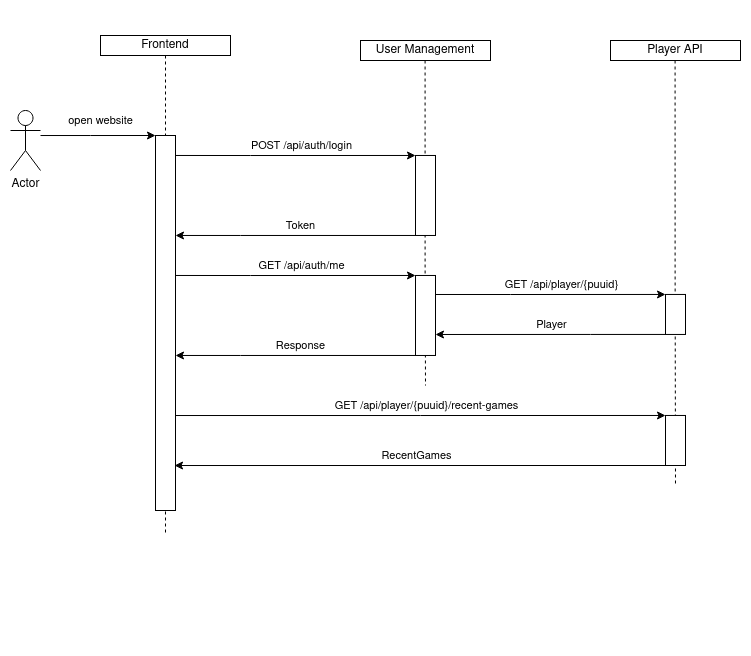
\includegraphics[width=\textwidth]{cdc-07-dynamic-get_own_data.drawio}
    \caption{Sequenzdiagramm für das Laden von Spielerdaten}
    \label{fig:load-data}
\end{figure}

In Abbildung~\ref{fig:load-data} ist der Ablauf gezeigt, welche Http Requests gesendet werden, wenn sich ein Spieler
der schon einen Account hat und dessen Spiele schon importiert sind, einloggt.


\subsection{Neuer Spieler importieren}

Um einen neuen Spieler zu importieren, wird eine Anfrage von dem Frontend an die Player-API gesendet.
Da diese Anfrage zustandslos ist, werden regelmäßig HTTP-Anfragen gesendet, um den aktuellen Import-Status
zu erhalten.
Diese Informationen werden im Frontend an den entsprechenden stellen dargestellt.
Im Player-API Service wird für den Import ein Backgroundtask gestartet, der über einen grpc Stream den Import im
Games Importer Service startet und die Anzahl der importierten Spiele streamt.

\graphic{cdc-07-import-player.drawio}{Flussdiagramm des Spieler imports}

\subsection{Spieler vergleichen}

Das Diagramm in Abbildung~\ref{fig:compare-diagram} stellt den Ablauf dar, wenn sich ein Spieler mit anderen Spielern vergleichen will.

\begin{figure}[H]
    \centering
    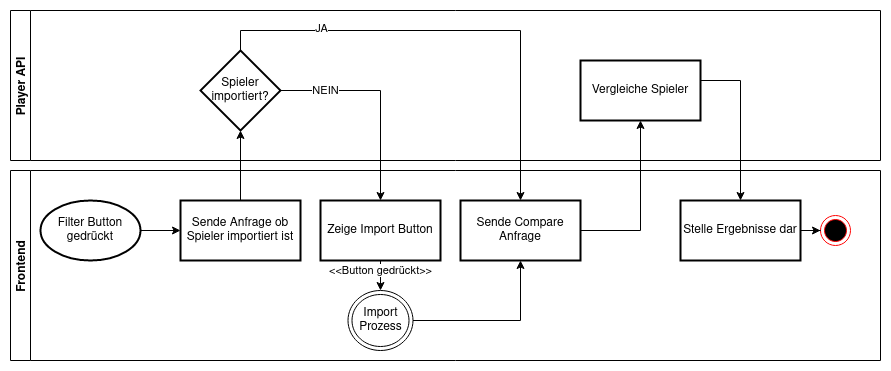
\includegraphics[width=\textwidth]{cdc-07-compare.drawio}
    \caption{Swimlane Diagramm zum Vergleich von Spielern}
    \label{fig:compare-diagram}
\end{figure}

\subsection{Error handling}
\subsubsection{Game importing}
Beim importieren des Spiels können wie in \ref{riot-api-libraries} bereits erklärt verschiedene Fehler auftreten. Damit Fehler, die von der Riot API kommen und meist nur temporär sind, nicht den Service zum Absturz bringen, werden alle API Aufrufe innerhalb einer try, except Anweisung ausgeführt. Sollte dann ein API Aufruf zu einem Fehler führen, so wird dieser bei Fehlern wie 503 - Service Unavailable wiederholt. Bei Fehlern, die nicht temporär sind (400 - Bad Request) wird der Request verworfen.\\
Auch die Datenbank kann Errors liefern, weshalb auch alle Datenbank Anfragen innerhalb von try, except Anweisung laufen. Tritt hierbei ein Fehler auf, so wird die komplette Anfrage die zu diesem geführt hat (zB das importieren eines Spiels) abgebrochen, so dass der Service weitere Anfragen verarbeiten kann. Wird ein Ablauf, wie das importieren eines Spiels unterbrochen, so wird dieser im nächsten update Durchlauf erneut versucht.

\subsubsection{Monitoring}

Um die Applikation zu monitoren, werden verschiedene Tools verwendet.

\textbf{sentry} (\href{https://sentry.io/}{https://sentry.io/}) wird verwendet, um Fehler zentral zu tracken und
Alerts zu verschicken.
Sentry wurde für alle Backend Services eingerichtet um einen Überblick über serverseitiges Fehlverhalten zu bekommen.

Um die Performance von Requests zu tracken, wird \textbf{SigNoz} (\href{https://signoz.io/}{https://signoz.io/}) verwendet.
Damit werden Traces für Anfragen erstellt, womit festgestellt werden kann wie lange Anfragen brauchen und welche Methode wie lange braucht.
Außerdem werden automatisch Datenbank Operationen gemessen, wodurch es möglich ist zwischen Applikationslogik
und Datenbank Operationen zu unterscheiden, wie in Abbildung~\ref{fig:signoz-traces} zu sehen ist.
\begin{figure}[H]
    \centering
    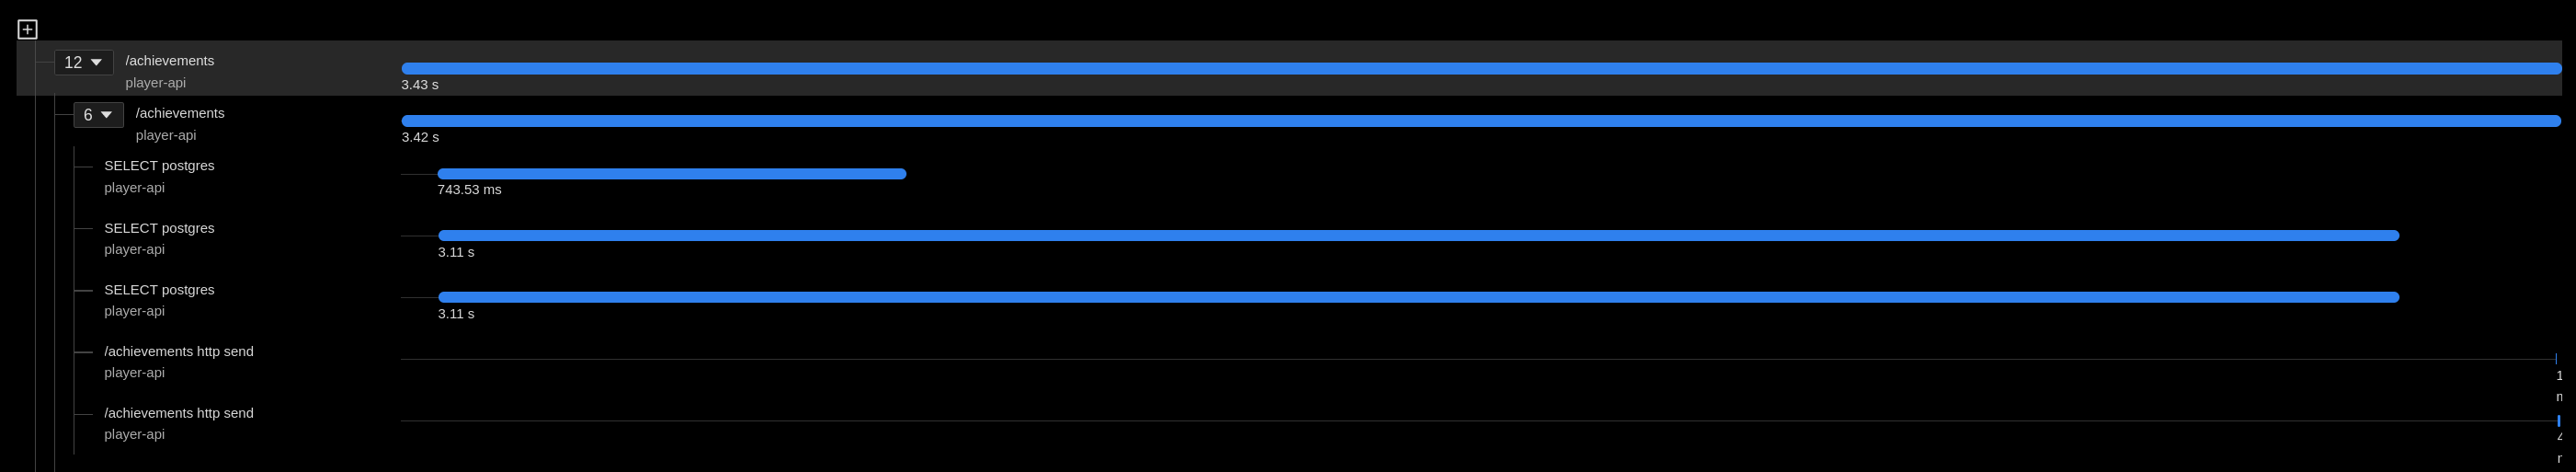
\includegraphics[width=\textwidth]{signoz_traces}
    \caption{Trace Details in SigNoz zu einem /achievements Request}
    \label{fig:signoz-traces}
\end{figure}
\section{Verteilungssicht}

In Abbildung~\ref{fig:deployment-diagram} ist eine Übersicht über das Deployment der Applikation und dazugehöriger
Services zu sehen.
\begin{figure}[H]
    \centering
    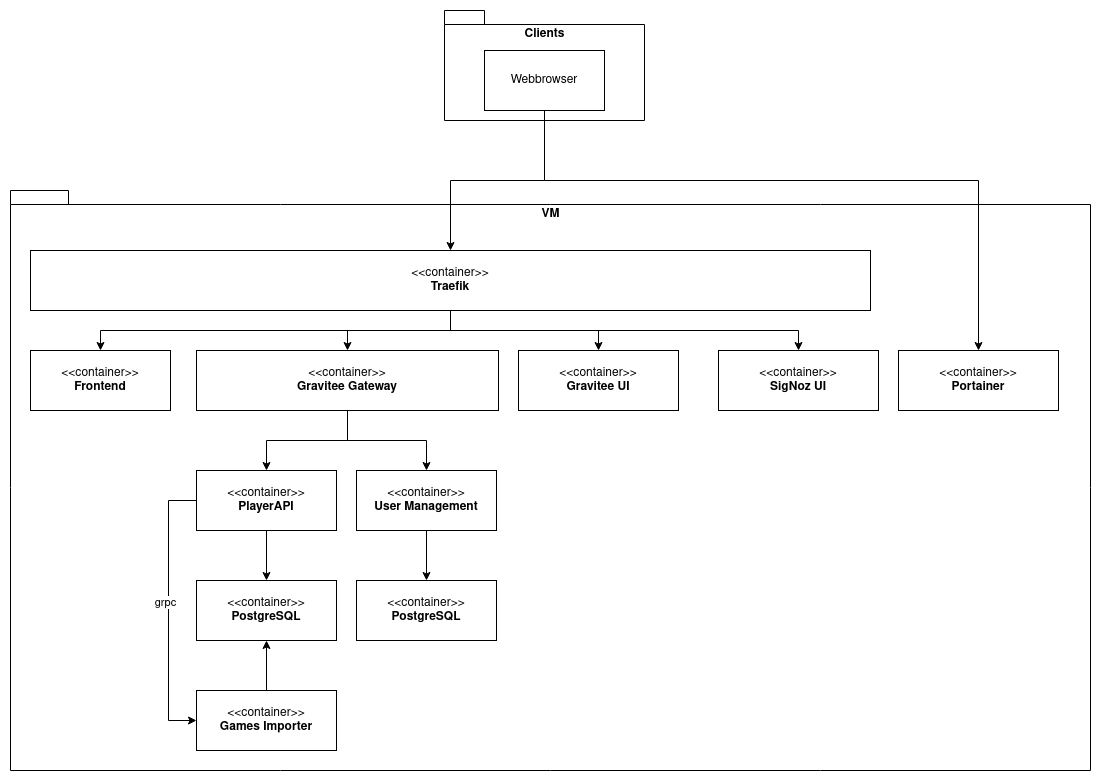
\includegraphics[width=\textwidth]{cdc-08-deployment-diagram.drawio}
    \caption{Deployment Diagramm}
    \label{fig:deployment-diagram}
\end{figure}

Die gesamte Applikation läuft innerhalb einer VM, wobei alles verdockert ist.
Das initiale Routing und Bereitstellen von Https Zertifikaten übernimmt Traefik (Edge Router).
So gibt es für jeden Teil eine eigene URL:
\begin{itemize}
    \item Frontend: lol-stats.de
    \item API (Gravitee Gateway): lol-stats.de/api
    \item Gravitee UI: api-ui.lol-stats.de
    \item SigNoz UI: tracing.lol-stats.de
    \item Grafana: grafana.lol-stats.de
\end{itemize}

Nur Portainer (Webseite zum Verwalten von Docker Stacks) ist direkt über einen Port erreichbar, weil es keine gute Idee ist Traefik in Portainer einzurichten
und gleichzeitig Portainer nur über Traefik erreichbar zu machen.
Alle API Anfragen werden über das Gravitee Gateway geleitet.
Gravitee ist eine API Management Software über die, die internen API Routen festgelegt werden.
Gravitee lässt sich über ein Webinterface in der Gravitee UI konfigurieren.
Die eingesammelten Traces lassen sich über ein Webinterface in der SigNoz UI anschauen.
Über Grafana (Datenvisualisierungstool) lassen sich die von Loki (Log-Aggregierung-Tool) eingesammelten Logs durchsuchen.

\section{Querschnittliche Konzepte}

\subsection{LoL Database ER-Diagram}
\graphic{LoLDatabase}{ER-Diagramm der LoL Datenbank}
In dieser Datenbank werden alle League of Legends bezogenen Daten gespeichert. Das sind alle Daten die dann auch im Frontend angezeigt werden. Die Daten werden vom Games Importer Service in die Datenbank geschrieben und dann von der Player API für das Frontend zur Verfügung gestellt.\\
Tabellen in der Datenbank:\\
\begin{itemize}
\item \textbf{Summoners:} Daten für einen Spieler
\item \textbf{Games:} Daten für einzelne Spiele
\item \textbf{Challenges:} Werte des Spieler in einer Challenge
\item \textbf{ChallengeClasses:} Verschiedene Challenges, die in der Challenges Tabelle auftauchen können, mit genauerer Beschreibung und Einteilung in Klassen
\item \textbf{SummonerSpells:} Klasse für Mapping von SummonerSpell IDs zu Name und Icon URL
\item \textbf{Champions:} Klasse für Mapping von Champion IDs zu Name und Icon URL
\item \textbf{Items:} Klasse für Mapping von Item IDs zu Name und Icon URL
\item \textbf{SummonerIcons:} Klasse für Mapping von Icon IDs zu URL
\item \textbf{Patches:} Hier wird gespeichert, welche Patches von League of Legends bereits in der Datenbank eingetragen wurden. Da mit jedem Patch z.B. neue Icons dazukommen, müssen die Tabellen nach jedem Patch geupdated werden. Nach dem update wird in dieser Tabelle festgehalten, wann die Datenbank für welchen Patch geupdated wurde.
\end{itemize}

\subsection{User Database ER-Diagramm}
\graphic{userbackend-db-er-schema}{ER-Diagramm der Datenbank des User Managements}
In der Datenbank des User Managements werden alle User-spezifische Daten gespeichert. Dazu gehören unter anderem auch die persönlichen Präferenzen des Benutzers. 
So werden hier die favorisierten Achievements und die ausgewählten Competitors auch mit abgespeichert. Außerdem werden hier die kreierten Token aller User abgespeichert.   

\subsection{User Management API Spezifikation}
\begin{figure}
  \centering
  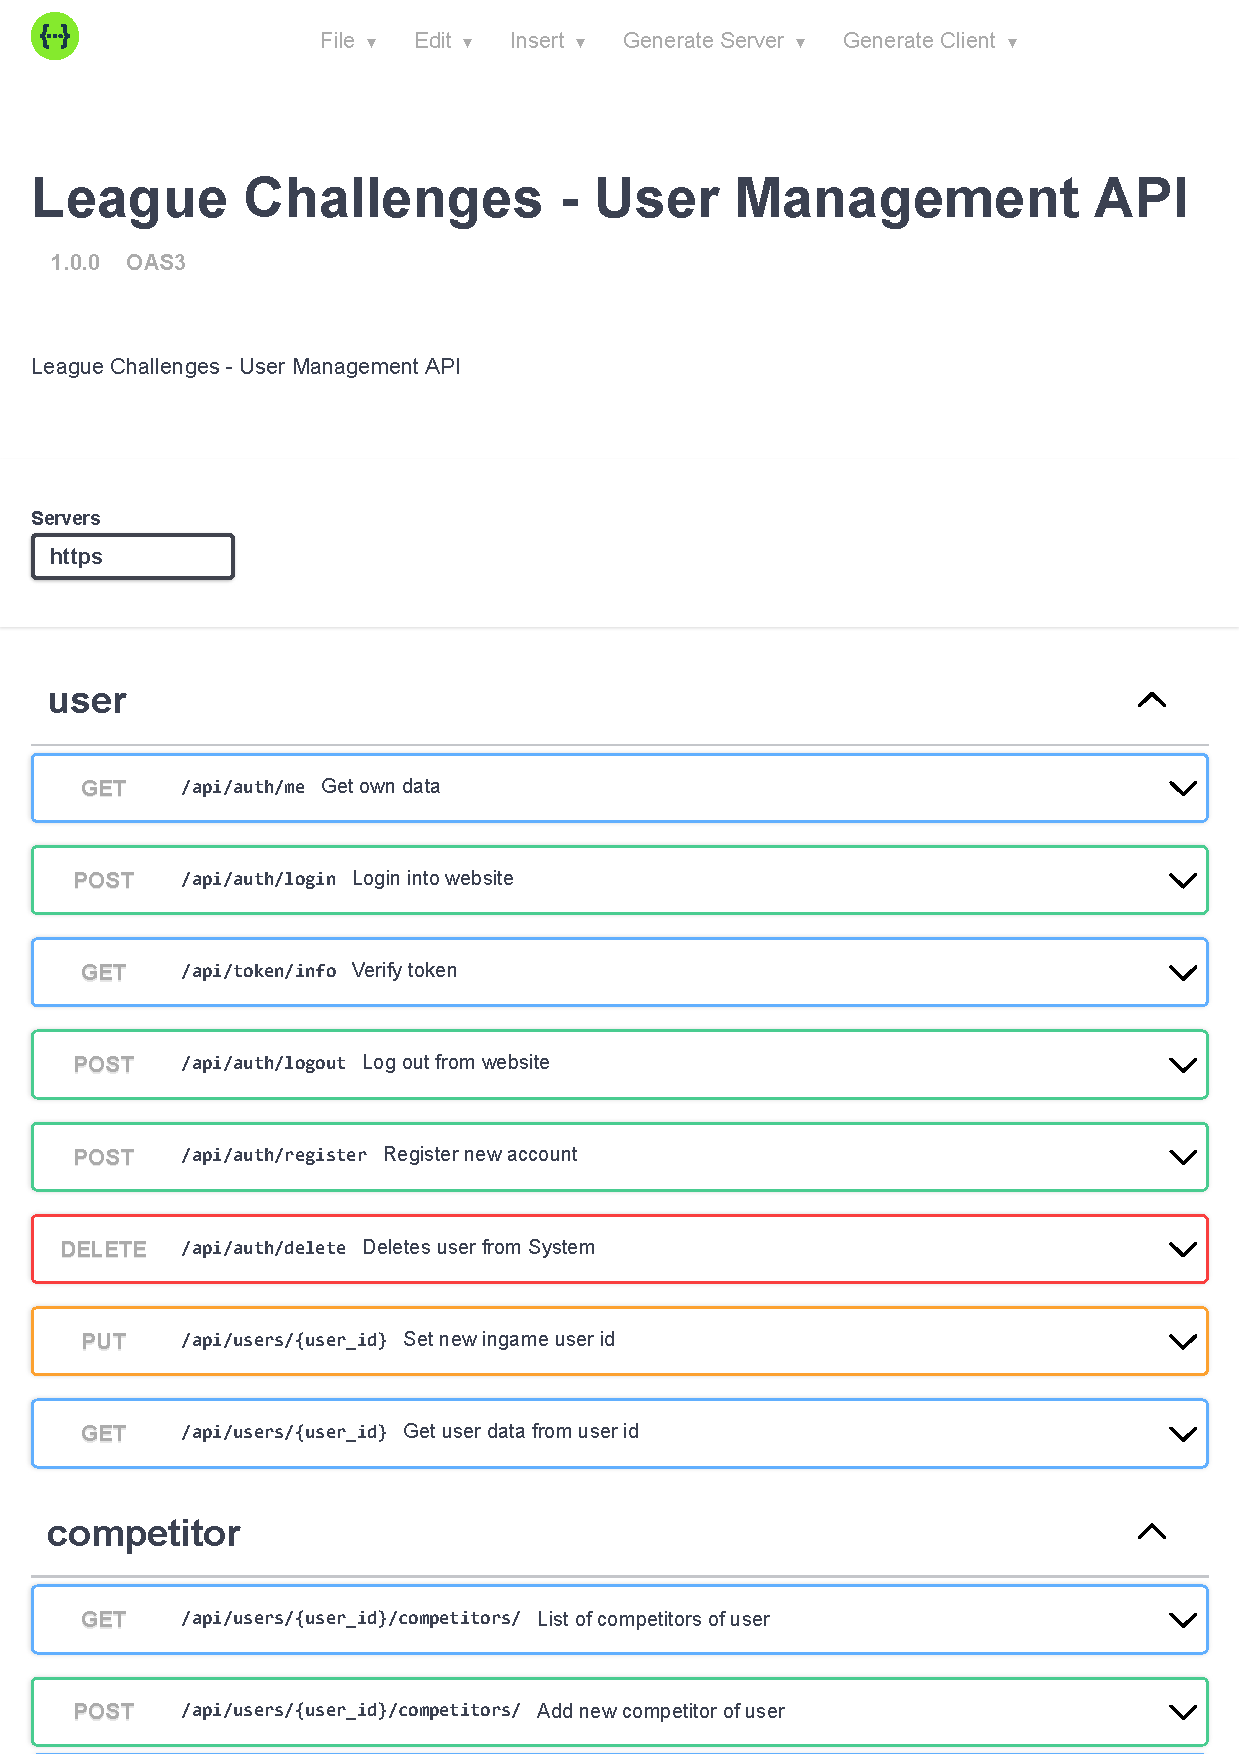
\includegraphics[width=1\textwidth, page=1]{images/pdfs/openapi-short.pdf}
  \caption{Kompakte Version der OpenApi vom User Management - Teil 1}
  \label{fig:compact_user_openapi_1}
\end{figure}
\begin{figure}
  \centering
  \includegraphics[width=1\textwidth, page=2]{images/pdfs/openapi-short.pdf}
  \caption{Kompakte Version der OpenApi vom User Management - Teil 2}
  \label{fig:compact_user_openapi_2}
\end{figure}

\subsection{Player API Spezifikation}
\todo{Player API Spec}

\subsection{GRPC Interface}
Damit der Import eines neuen Spieler angefragt werden kann, muss eine Kommunikation zwischen Frontend und dem Games Importer Service bestehen. Das Frontend kommuniziert nur mit der PlayerAPI, welche die Anfrage dann an den Games Importer Service weiterleiten muss.\\
Da der Player API Service und der Games Importer Service beide in Pyton geschrieben wurden, kann diese Kommunikation über GRPC erfolgen, welches es der PlayerAPI erlaubt über einen Protocol Request die Import Funktion des Game Importers aufzurufen.\\ % TODO Tim: für grps müssen Applikationen nicht in gleicher Sprache geschrieben sein. Grund war eher, dass grpc Streaming erlaubt
Die Schnittstelle wird in einer .proto Datei definiert:

\begin{lstlisting}
syntax = "proto3";

service Importer {
  rpc import_player (ImportRequest) returns (stream ImportReply) {}
}

message ImportRequest {
  string puuid = 1;
}

message ImportReply {
  int32 games_imported = 1;
  int32 total_games = 2;
}
\end{lstlisting}
Der Request beinhaltet hierbei die ID des zu importierenden Spielers und die Reply den aktuellen Fortschritt des Vorgangs. Die Reply wird solange gesendet, bis der Spieler vollständig importiert wurde.\\
Mithilfe dieser Datei werden dann die nötigen Python Klassen generiert. In der \textit{PlayerImportRequest.py} wird dann die \textit{import\_player(request, context)} Methode implementiert, welche dann beim erhalten eines Requests aufgerufen wird und im request Parameter die ID des Spieler erhält. Dann kann der Games Importer diesen importieren und mittels eines \textit{yield} Statements in der \textit{import\_player()} Funktion die Replies an die Player API senden.

\subsection{Zentrales Logging}

Um das Debuggen im Fehlerfall zu vereinfachen gibt es es zentrales Logging.
Die Logs aller Services werden zentral von Loki eingesammelt und gespeichert.
Die Logs werden über ein Docker Plugin direkt an Loki gesendet.
Über Grafana lassen sich die Logs mit der Query Sprache Logql durchsuchen.
So können zum Beispiel alle Logs eines Accounts im Games Importer Service angezeigt werden:

\begin{lstlisting}
  {compose_service="riot-api-connector"} |= `'accountId': 'P90cNvGn`
\end{lstlisting}

Das Ergebnis ist in Abbildung~\ref{fig:logging} zu sehen.
Oben wird auf einer Zeitachse dargestellt, wann, wie viele Logs gefunden werden.
Darunter sind alle gefundenen Logzeilen zu sehen.
Logzeilen können ausgeklappt werden, um weitere Metainformationen zu sehen.

\begin{figure}
    \centering
    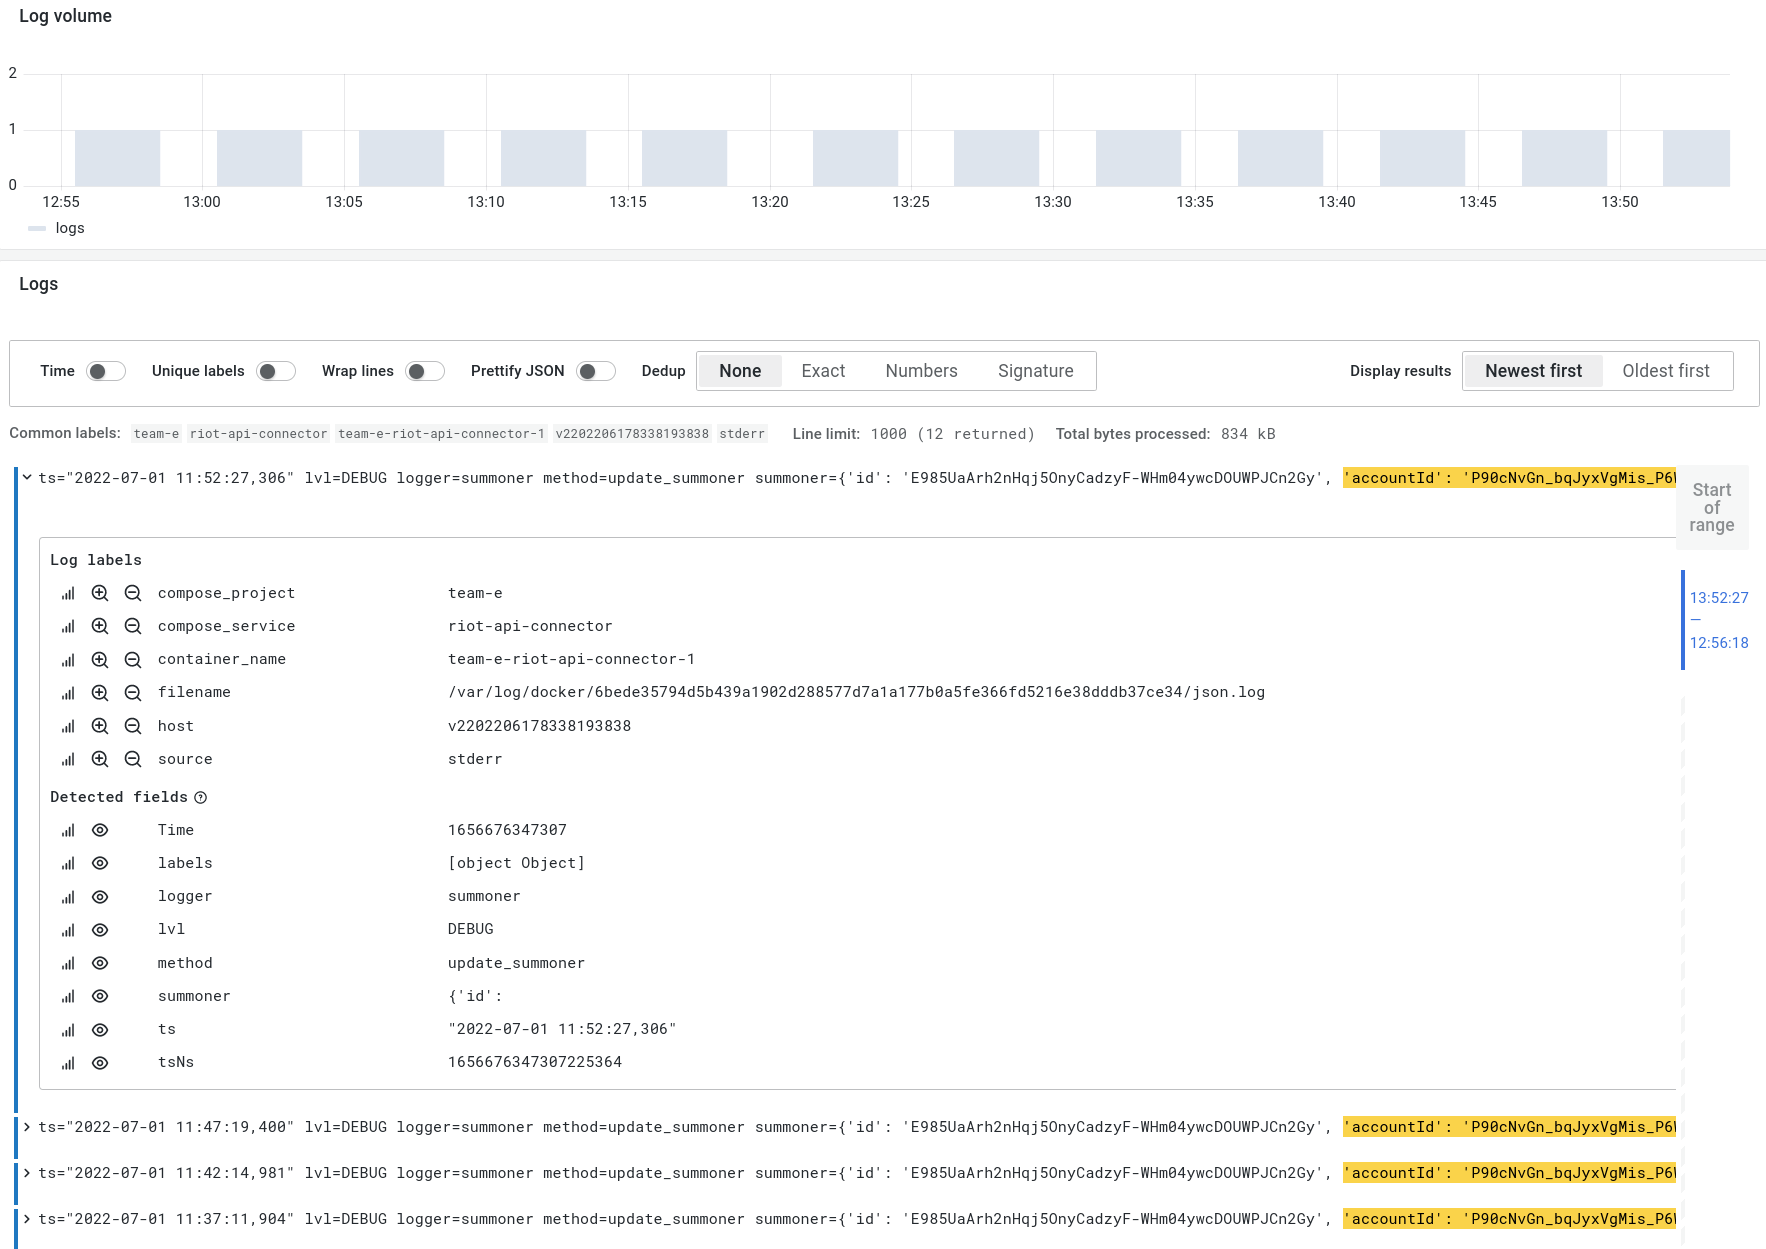
\includegraphics[width=\textwidth]{images/logging}
    \caption{Ergebnis des Logging Queries}
    \label{fig:logging}
\end{figure}
\section{Architekturentscheidungen}
\todo{Architekturentscheidungen}


\section{Qualtiy}
\section{Risiken und technische Schulden}
Potential problems, known technical risks, technical debt

\subsection{Database Performance}

Derzeit wird als Datenbankmanagementsystem "PostgreSQL" verwendet. In Kombination mit dieser und der gewählten Architektur verarbeitet das System die Anfragen und Berechnungen zuverlässig.
Jedoch kann es zu Performance-Problemen kommen, sobald die Softwarelösung von deutlich mehr Nutzer:innen verwendet wird. Der Grund dafür ist das ständige Wachsen der "LoL-Datenbank", wodurch die Abfrage und
die Berechnungen der Achievements langsamer werden. Hierfür müsste die Architektur so angepasst werden, dass eine bessere Skalierbarkeit des Datenbankmanagementsystems möglich ist.

\subsection{Riot API Ratelimits}
Wie bereits in \ref{riot-api-ratelimits} beschrieben, hat der momentan verwendete Development API Key geringe Ratelimits. Sollte die Website öffentlich zugänglich gemacht werden, muss zuerst ein Product API Key beantragt werden, was voraussetzt, dass das Produkt von Riot hierfür akzeptiert wird. Ist das nicht der Fall, so kann die Website nicht öffentlich zugänglich gemacht werden.

\subsection{Changes in Riot API}
Die Endpoints der Riot API verändern sich immer wieder. So wurde z.B. vor ein paar Monaten der alte Match-V4 Endpoint durch den neueren Match-V5 Endpoint ersetzt. Da für die Kommunikation mit der Riot API externe Libraries (Cassiopeia, Riot Watcher) verwendet werden, ist das Produkt momentan davon abhängig, dass auch diese dann geupdated werden.
Außerdem müssten die Änderungen dann im Games Importer Service ebenfalls eingebaut werden.\\ Sollten die Libraries nicht geupdated werden, so müsste man auf eine neue Library umsteigen, was viele Code Änderugnen bedeuten würde, oder einen eigenen Wrapper für die Verbindung mit der Riot API schreiben.

\subsection{Sicherheit}

Derzeit ist eine Authentifizierung implementiert, die mit Hilfe von JWT-Zugriffstokens bestimmte Seiten vor unbefugten Zugriff schützen.
Jedoch ist dies bei anderen API-Endpunkten ('Player-Backend') nicht der Fall. Ebenso existiert keine Zugriffskontrolle zwischen den
einzelnen Microservice-Diensten, um zu verifizieren, dass der Anfragende befugt ist. Hierfür können Zertifikate, die jeweils ein
Dienst besitzt, die dienstübergreifende Kommunikation mehr Sicherheit bieten. Ebenso wird dadurch die Kommunikation untereinander
verschlüsselt.

Ebenso fehlt ein Ratenlimit im Frontend beziehungsweise im Backend der einzelnen Dienste. Dadurch kann ein Denial-of-Service-Angriffe (DoS)
nicht verhindert werden oder ungewollte Auslastung der Netzwerkbandbreite. Dies ist vor allem bei der Schnittstelle kritisch, die für das 
Importieren von Spieler-Daten verantwortlich ist. Aufgrund der rechenintensiven Berechnung und Importierung der Spielerdaten kann 
eine erhöhte Auslastung zur Unstabilität des Dienstes führen.
\section{Glossary}


	
\end{document}